\documentclass{article}
\usepackage{graphicx} % Required for inserting images

\usepackage[square,sort,comma,numbers]{natbib}
\usepackage{amsmath} % Required for some math elements 

\usepackage{cmap}
\usepackage[T2A]{fontenc}
\usepackage[utf8x]{inputenc}
\usepackage[english, russian]{babel}

\usepackage{xcolor}
\usepackage[left=2cm,right=2cm,
    top=2cm,bottom=2cm,bindingoffset=0cm]{geometry}

\title{Lab1_MatStat}
\author{ksenerem03 }
\date{February 2023}

\begin{document}

\begin{titlepage}
\begin{center}
\textsc{Санкт-Петербургский политехнический университет\\Петра Великого\\[5mm]
Физико-механический институт\\[2mm]
Кафедра «Прикладная математика»}

\vfill

\textbf{Отчет\\по лабораторной работе №1\\по дисциплине\\ «Математическая статистика»
\\[26mm]
}
\end{center}

\vspace{6em}

\newbox{\lbox}
\savebox{\lbox}{\hbox{Еремина Ксения Игоревна}}
\newlength{\maxl}
\setlength{\maxl}{\wd\lbox}
\hfill\parbox{14cm}{
\hspace*{5cm}\hspace*{-5cm}Выполнила студентка \hfill\hbox to\maxl{ }\\
\hspace*{5cm}\hspace*{-5cm}группы 5030102/00101\hfill\hbox to\maxl{Еремина Ксения Игоревна\hfill}\\
\hspace*{5cm}\hspace*{-5cm}Проверил \hfill\hbox to\maxl{ }\\
\hspace*{5cm}\hspace*{-5cm}Доцент, к.ф.-м.н. \hfill\hbox to\maxl{Баженов Александр Николаевич\hfill}\\}
\\


\vspace{\fill}


\begin{center}
 Санкт-Петербург\\2023 г.
\end{center}
\end{titlepage}

\newpage

\tableofcontents
\newpage

\listoffigures
\newpage

\listoftables
\newpage
 
%----------------------------------------------------------------------------------------
%	SECTION 1
%----------------------------------------------------------------------------------------

\section{Постановка задачи}
Для 4 распределений:

\begin{itemize}
    \item Нормальное распределение $N(x,0,1)$
    \item Распределение Коши $C(x,0,1)$
    \item Распределение Пуассона $P(k,10)$
    \item Равномерное распределение $U(x,-\sqrt{3},\sqrt{3})$
\end{itemize}
\begin{enumerate}
    \item Сгенерировать выборки размером 10, 50 и 1000 элементов.
    Построить на одном рисунке гистограмму и график плотности распределения.
    \item Сгенерировать выборки размером 10, 100 и 1000 элементов.
    Для каждой выборки вычислить следующие статистические характеристики положения данных: $\overline{x}, med \; x, z_R, z_Q, z_{tr}$. Повторить такие вычисления 1000 раз для каждой выборки и найти среднее характеристик положения и их квадратов:
    \begin{equation}
    E(z)=\overline{z}
    \end{equation}
    Вычислить оценку дисперсии по формуле:
    \begin{equation}
    D(z)=\overline{z^2}-\overline{z}^2
    \end{equation}
    Представить полученные данные в виде таблиц.
    \item Сгенерировать выборки размером 20 и 100 элементов. Построить для них боксплот Тьюки. Для каждого распределения определить долю выбросов экспериментально (сгенерировав выборку, соответствующую распределению 1000 раз, и вычислив среднюю долю выбросов) и сравнить с результатами, полученными теоретически.
    \item Сгенерировать выборки размером 20, 60 и 100 элементов. Построить на них эмпирические функции распределения и ядерные оценки плотности распределения на отрезке $[−4; 4]$ для непрерывных распределений и на отрезке $[6; 14]$ для распределения Пуассона.


\end{enumerate}

\newpage

\section{Теория}

\subsection{Рассматриваемые распределения}
Плотности:
\begin{itemize}
  \item Нормальное распределение
  
  \begin{equation}
      N(x, 0, 1) = \tfrac{1}{\sqrt{2\pi}}e^{-\tfrac{x^2}{2}}
  \end{equation}
  
  \item Распределение Коши
  
   \begin{equation}
      C(x, 0, 1) = \dfrac{1}{\pi}\dfrac{1}{x^2+1}
  \end{equation}
  
  \item Распределение Пуассона
  
  \begin{equation}
      P(k, 10) = \tfrac{10^k}{k!}e^{-10}
  \end{equation}
  
  \item Равномерное распределение
  
    \begin{equation}
      U(x, -\sqrt{3}, \sqrt{3}) =
        \begin{cases} 
            \;\; \dfrac{1}{2\sqrt{3}} \;\;\;\; \text{при} \;\;\;\; x \in [-\sqrt{3}, \sqrt{3}]\\
            \,\,\,\:\;\; 0 \;\;\;\;\;\;\; \text{при} \;\;\;\; x \not\in [-\sqrt{3}, \sqrt{3}]
        \end{cases}
  \end{equation}
  
\end{itemize}

\subsection{Гистограмма}

\subsubsection{Построение гистограммы}
Множество значений, которое может принимать элемент выборки, разбивается на несколько интервалов. Чаще всего эти интервалы берут одинаковыми, но это не является строгим требованием. Эти интервалы откладываются
на горизонтальной оси, затем над каждым рисуется прямоугольник. Если
все интервалы были одинаковыми, то высота каждого прямоугольника пропорциональна числу элементов выборки, попадающих в соответствующий
интервал. Если интервалы разные, то высота прямоугольника выбирается
таким образом, чтобы его площадь была пропорциональна числу элементов
выборки, которые попали в этот интервал [1].

\subsection{Вариационный ряд}
Вариационным ряд - последовательность элементов выборки, расположенных в неубывающем порядке. Одинаковые элементы повторяются [2, с. 409].

\subsection{Выборочные числовые характеристики}

\subsubsection{Характеристики положения}

\begin{itemize}
  \item Выборочное среднее
  
  \begin{equation} \label{eq:mean}
    \overline{x} = \tfrac{1}{n}\sum\limits_{i=1}^n x_i
  \end{equation}
  
  \item Выборочная медиана
  
  \begin{equation} \label{eq:med}
    med \: x = 
    \begin{cases} 
        \;\;\;\;\;\;\; x_{(l+1)} \:\;\;\;\;\;\;\;\;\; \text{при} \;\;\;\; n = 2l + 1\\
        \;\; \dfrac{x_{(l)} + x_{(l+1)}}{2} \;\;\;\; \text{при} \;\;\;\; n = 2l
    \end{cases}
  \end{equation}
  
  \item Полусумма экстремальных выборочных элементов
  
  \begin{equation} \label{eq:zR}
    z_R = \dfrac{x_{(1)} + x_{(n)}}{2}
  \end{equation}
  
  \item Полусумма квартилей
  
  Выборочная квартиль $z_p$ порядка $p$ определяется формулой
  
   \begin{equation}
    z_p =
    \begin{cases}
        \;\; x_{([np]+1)} \;\;\;\; \text{при} \;\; np \;\; \text{дробном},\\
        \;\;\;\;\; x_{(np)} \,\:\;\;\;\;\; \text{при} \;\; np \;\; \text{целом}.
    \end{cases}
  \end{equation}
  
  Полусумма квартилей
  
  \begin{equation} \label{eq:zQ}
    z_Q = \dfrac{z_{1/4} + z_{3/4}}{2}
  \end{equation}
  
  \item Усечённое среднее
  
  \begin{equation} \label{eq:zTr}
    z_{tr} = \tfrac{1}{n-2r}\sum\limits_{i=r+1}^{n-r} x_{(i)}, \;\;\;\; r \approx \dfrac{n}{4}
  \end{equation}
  
\end{itemize}

\subsubsection{Характеристики рассеяния}

Выборочная дисперсия

\begin{equation}
    D = \tfrac{1}{n}\sum\limits_{i=1}^{n} (x_i - \overline{x})^2
\end{equation}

\subsection{Боксплот Тьюки}

\subsubsection{Построение}

Границами ящика служат первый и третий квартили, линия в середине ящика --- медиана. Концы усов --- края статистически значимой выборки (без выбросов). Длину «усов»:

\begin{equation} \label{eq:boundBoxplot}
    X_1 = Q_1 - \dfrac{3}{2}(Q_3 - Q_1), \;\; X_2 = Q_3 + \dfrac{3}{2}(Q_3 - Q_1),
\end{equation}

где $X_1$ --- нижняя граница уса, $X_2$ --- верхняя граница уса, $Q_1$ --- первый квартиль, $Q_3$ --- третий квартиль.

Данные, выходящие за границы усов (выбросы), отображаются на графике в виде маленьких кружков .

\subsection{Теоретическая вероятность выбросов}

Можно вычислить теоретические первый и третий квартили распределений $Q_1^\text{т}$ и $Q_3^\text{т}$ соответственно. По формуле \eqref{eq:boundBoxplot} - теоретические нижнюю и верхнюю границы уса $X_1^\text{т}$ и $X_2^\text{т}$. Выбросы - величины $x$:

\begin{equation}
    \left[ 
        \begin{gathered} 
            x < X_1^\text{т}\\ 
            x > X_2^\text{т}\\ 
        \end{gathered} 
    \right.
\end{equation}

Теоретическая вероятность выбросов:

\begin{itemize}
    \item для непрерывных распределений
    \begin{equation} \label{eq:probTheorCont}
    P_\text{в}^\text{т} = P(x < X_1^\text{т}) + P(x > X_2^\text{т}) = F(X_1^\text{т}) + \Big(1 - F(X_2^\text{т})\Big)
    \end{equation}
    \item для дискретных распределений
    \begin{equation} \label{eq:probTheorDisc}
    P_\text{в}^\text{т} = P(x < X_1^\text{т}) + P(x > X_2^\text{т}) = \Big(F(X_1^\text{т}) - P(x = X_1^\text{т})\Big) + \Big(1 - F(X_2^\text{т})\Big)
    \end{equation}
\end{itemize}
Выше $F(X) = P(x \le X)$ - функция распределения.

\subsection{Эмпирическая функция распределения}

\subsubsection{Статистический ряд}
Статистическим ряд – последовательность различных элементов выборки $z_1, z_2, ..., z_k,$ расположенных в возрастающем порядке с указанием частот $n_1, n_2, ..., n_k,$ с которыми эти элементы содержатся в выборке. Обычно записывается в виде таблицы.

\subsubsection{Эмпирическая функция распределения}
Эмпирической (выборочной) функцией распределения (э. ф. р.) называется относительная частота события $X < x$, полученная по данной выборке:

\begin{equation}
    F_n^*(x) = P^*(X < x).
\end{equation}

\subsubsection{Нахождение э. ф. р.}

Для получения относительной частоты $P^*(X < x)$ просуммируем в статистическом ряде, построенном по данной выборке, все частоты $n_i$, для которых элементы $z_i$ статистического ряда меньше $x$. Тогда $P^*(X < x) = \tfrac{1}{n}\sum\limits_{z_i < x}n_i$. Получаем

\begin{equation}
    F^*(x) = \tfrac{1}{n}\sum\limits_{z_i < x}n_i.
\end{equation}

$F^*(x)$ --- функция распределения дискретной случайной величины $X^*$, заданной таблицей распределения

\begin{table}[h!]
\begin{center}
\begin{tabular}{|c|c|c|c|c|}
\hline
$X^*$ & $z_1$ & $z_2$ & $...$ & $z_k$ \\
\hline
$P$ & $\dfrac{n_1}{n}$ & $\dfrac{n_2}{n}$ & $...$ & $\dfrac{n_k}{n}$ \\
\hline
\end{tabular}
\end{center}
\caption{Таблица распределения}
\end{table}

Эмпирическая функция распределения является оценкой, т. е. приближённым значением, генеральной функции распределения

\begin{equation}
    F_n^*(x) \approx F_X(x).
\end{equation}

\subsection{Оценки плотности вероятности}

\subsubsection{Определение}
Оценкой плотности вероятности $f(x)$ называется функция $\widehat{f}(x)$, построенная на основе выборки, приближённо равная $f(x)$

\begin{equation}
    \widehat{f}(x) \approx f(x).
\end{equation}

\subsubsection{Ядерные оценки}
Представим оценку в виде суммы с числом слагаемых, равным объёму выборки:

\begin{equation}
    \widehat{f}_n(x) = \tfrac{1}{nh_n}\sum\limits_{i=1}^n K\left( \tfrac{x - x_i}{h_n} \right).
\end{equation}

Здесь функция $K(u)$, называемая ядерной (ядром), непрерывна и является плотностью вероятности, $x_1, \, ... \: , x_n$ --- элементы выборки, $\{h_n\}$ --- любая последовательность положительных чисел, обладающая свойствами

\begin{equation}
    h_n \underset{n \to \infty}{\longrightarrow} 0; \qquad \dfrac{h_n}{n^{-1}} \underset{n \to \infty}{\longrightarrow} \infty.
\end{equation}

Такие оценки называются непрерывными ядерными\\

Гауссово (нормальное) ядро:

\begin{equation}
    K(u) = \tfrac{1}{\sqrt{2\pi}}e^{-\tfrac{u^2}{2}}.
\end{equation}

Правило Сильвермана 

\begin{equation}
    h_n = 1.06\hat{\sigma}n^{-1/5},
\end{equation}

где $\hat{\sigma}$ - выборочное стандартное отклонение.

\newpage

\section{Реализация}

Лабораторная работа выполнена на языке Python версии 3.8 в среде разработки PyCharm.
Использовались дополнительные библиотеки:
\begin{itemize}
    \item scipy
    \item numpy
    \item matplotlib
    \item math
\end{itemize}

\newpage

\section{Результаты}

\subsection{Гистограммы и графики плотности распределения}

\begin{figure}[!ht]
\begin{center}
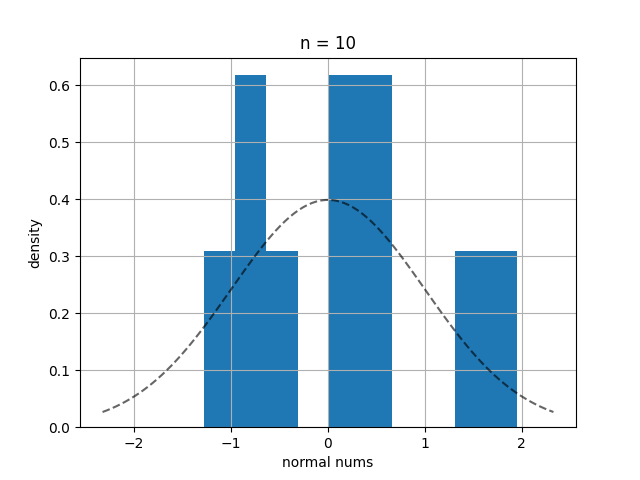
\includegraphics[scale=0.35]{NormalDistnormal10.png}
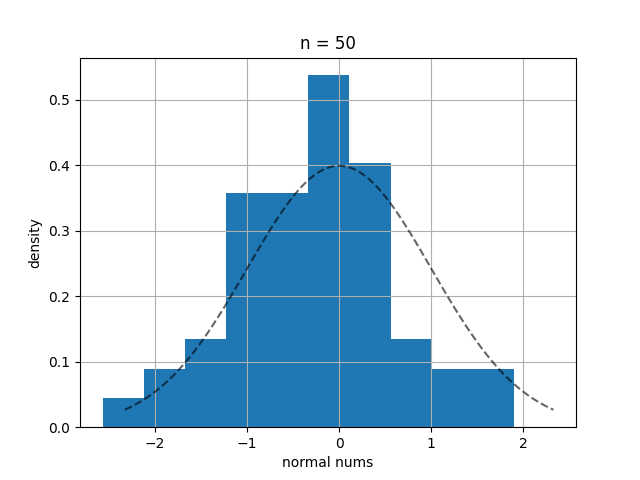
\includegraphics[scale=0.35]{NormalDistnormal50.png}
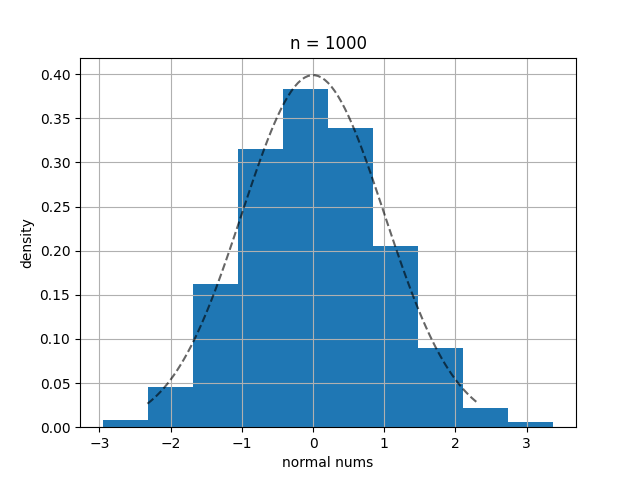
\includegraphics[scale=0.35]{NormalDistnormal1000.png}
\caption{Нормальное распределение}\label{figure1}
\end{center}
\end{figure}

\begin{figure}[!ht]
\begin{center}
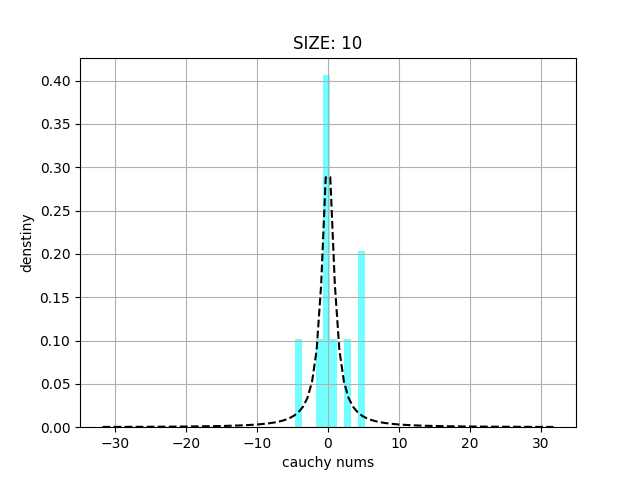
\includegraphics[scale=0.35]{CauchyDistcauchy10.png}
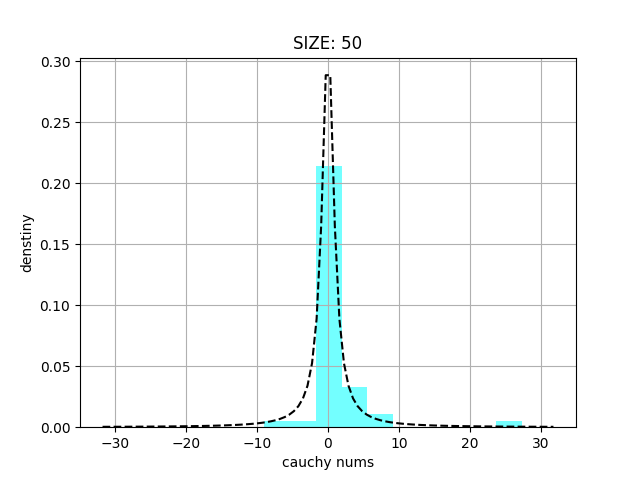
\includegraphics[scale=0.35]{CauchyDistcauchy50.png}
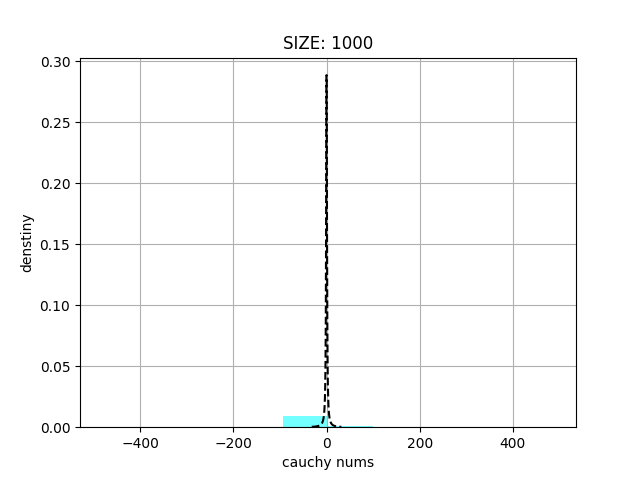
\includegraphics[scale=0.35]{CauchyDistcauchy1000.png}
\caption{Распределение Коши}\label{figure2}
\end{center}
\end{figure}

\begin{figure}[!ht]
\begin{center}
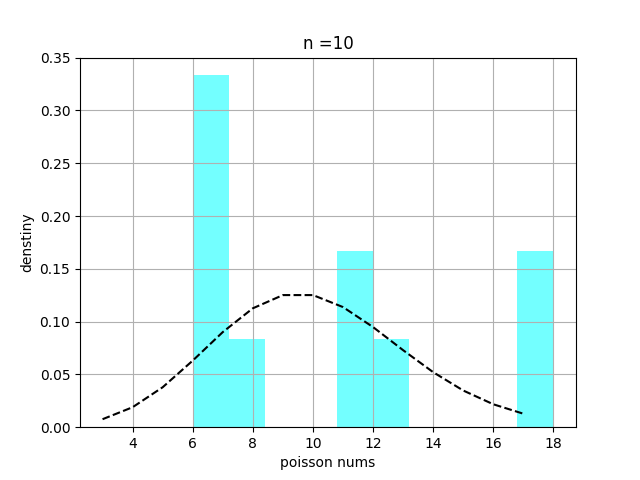
\includegraphics[scale=0.35]{PoissonDistpoisson10.png}
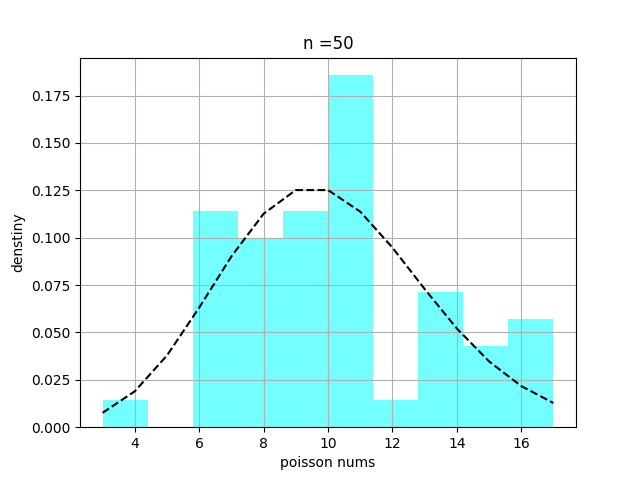
\includegraphics[scale=0.35]{PoissonDistpoisson50.png}
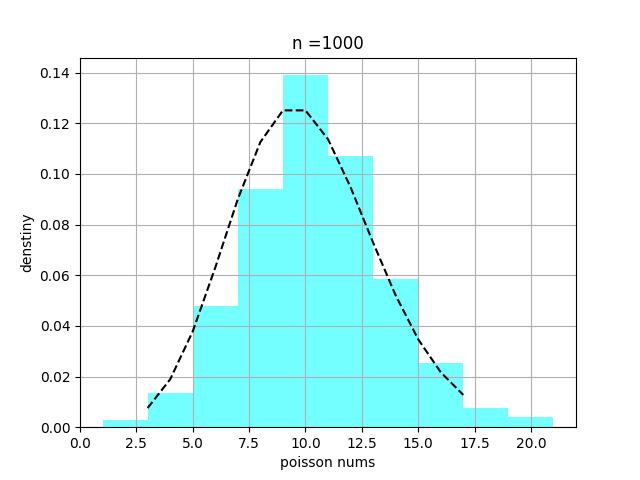
\includegraphics[scale=0.35]{PoissonDistpoisson1000.png}
\caption{Распределение Пуассона}\label{figure4}
\end{center}
\end{figure}

\begin{figure}[!ht]
\begin{center}
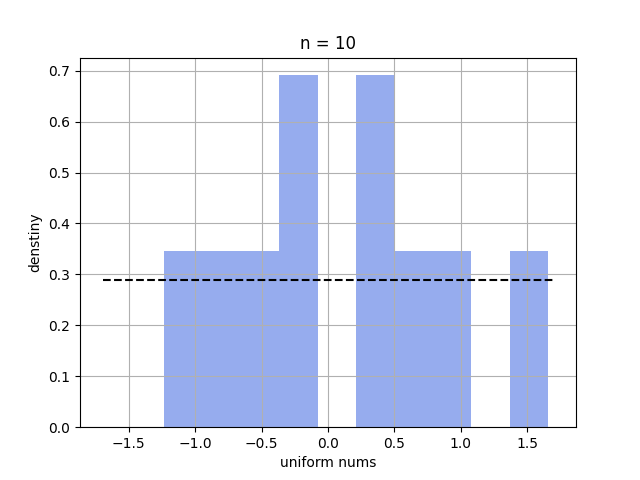
\includegraphics[scale=0.35]{UniformDistuniform10.png}
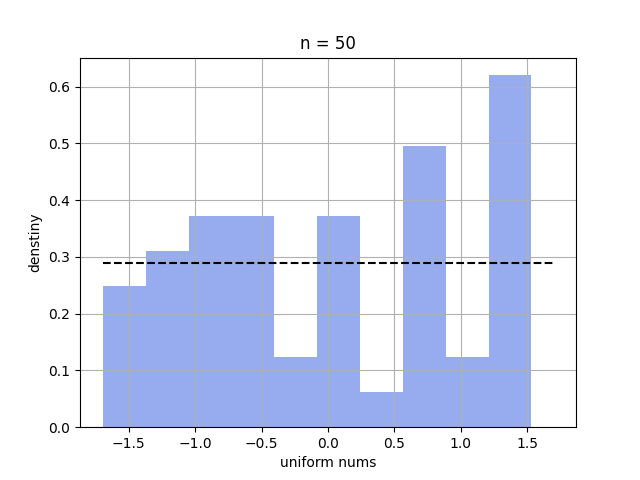
\includegraphics[scale=0.35]{UniformDistuniform50.png}
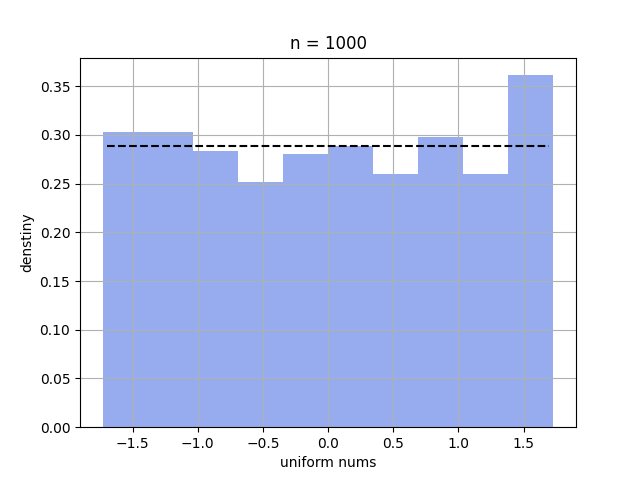
\includegraphics[scale=0.35]{UniformDistuniform1000.png}
\caption{Равномерное распределение}\label{figure5}
\end{center}
\end{figure}
~\\
~\\
~\\
~\\
~\\
~\\
~\\
~\\
~\\



\subsection{Характеристики положения и рассеяния}

\begin{table}[h!]
\begin{center}
\begin{tabular}{|c|c|c|c|c|c|}
\hline
 & <x> & med x & zR & zQ & Ztr \\
 \hline
n=10 & & & & & \\
\hline
Normal E(z) & 0.000826 & 0.007095 & -0.002096 & 0.311883 & 0.276208 \\
\hline
Normal D(z) & 0.103509 & 0.142529 & 0.185601 & 0.1278 & 0.11815 \\
\hline
E(z) $\pm \sqrt{D(z)}$ & [-0.32;0.32] & [-0.37;0.38] & [-0.43;0.42] & [-0.05;0.67] & [-0.07;0.62] \\
\hline
n=100 & & & & & \\
\hline
Normal E(z) & 0.001901 & -0.000416 & 0.008904 & 0.018747 & 0.027085 \\
\hline
Normal D(z) & 0.010657 & 0.017139 & 0.095083 & 0.013155 & 0.012952 \\
\hline
E(z) $\pm \sqrt{D(z)}$ & [-0.10;0.11] & [-0.13;0.13] & [-0.30;0.32] & [-0.10;0.13] & [-0.09;0.14] \\
\hline
n=1000 & & & & & \\
\hline
Normal E(z) & 0.000169 & 0.000363 & 0.00097 & 0.001855 & 0.002716 \\
\hline
Normal D(z) & 0.00102 & 0.001522 & 0.058933 & 0.001288 & 0.001181 \\
\hline
E(z) $\pm \sqrt{D(z)}$ & [-0.03;0.03] & [-0.04;0.04] & [-0.24;0.24] & [-0.03;0.04] & [-0.03;0.04] \\
\hline

\end{tabular}
\caption{Нормальное распределение}
\label{tabular:timesandtenses}
\end{center}
\end{table}

    
\begin{table}[h!]
\begin{center}
\begin{tabular}{|c|c|c|c|c|c|}
\hline
 & <x> & med x & zR & zQ & Ztr \\
 \hline
n=10 & & & & & \\
\hline
Cauchy E(z) & -1.525697 & -0.020663 & -7.536897 & 1.05869 & 0.655965 \\
\hline
Cauchy D(z) & 739.187373 & 0.360723 & 18396.710165 & 5.032606 & 1.38404 \\
\hline
E(z) $\pm \sqrt{D(z)}$ & [-28.71;25.66] & [-0.62;0.58]  & [-143.17;128.10] & [-1.18;3.30] & [-0.52;1.83] \\
\hline
n=100 & & & & & \\
\hline
Cauchy E(z) & -0.284393 & -0.004505 & -13.293061 & 0.035872 & 0.041822 \\
\hline
Cauchy D(z) & 275.816143 & 0.025083 & 673320.932083 & 0.051133 & 0.026515 \\
\hline
E(z) $\pm \sqrt{D(z)}$ & [-16.90;16.32] & [-0.16;0.15] & [-833.85;807.27] & [-0.19;0.26] & [-0.12;0.20] \\
\hline
n=1000 & & & & & \\
\hline
Cauchy E(z) & 0.212424 & 0.000775 & 121.549193 & 0.004567 & 0.004748 \\
\hline
Cauchy D(z) & 1023.878903 & 0.002212 & 253459308.779892 & 0.004833 & 0.002351 \\
\hline
E(z) $\pm \sqrt{D(z)}$ & [-31.79;32.21] & [-0.05;0.05] & [-15798.86;16041.95] & [-0.06;0.07] & [-0.04;0.05] \\
\hline
\end{tabular}
\caption{Распределение Коши}
\label{tabular:timesandtenses}
\end{center}
\end{table}






\begin{table}[h!]
\begin{center}
\begin{tabular}{|c|c|c|c|c|c|}
\hline
 & <x> & med x & zR & zQ & Ztr \\
\hline
n=10 & & & & & \\
\hline
Poisson E(z) & 9.9671 & 9.847 & 10.2465 & 10.916 & 10.7555 \\
\hline
Poisson D(z) & 0.957568 & 1.375591 & 1.820988 & 1.318944 & 1.222914 \\
\hline
E(z) $\pm \sqrt{D(z)}$ & [8.99;10.95] & [8.67;11.02] & [8.90;11.60] & [9.77;12.06] & [9.65;11.86] \\
\hline
n=100 & & & & & \\
\hline
Poisson E(z) & 10.00494 & 9.843 & 10.9445 & 9.971 & 9.94612 \\
\hline
Poisson D(z) & 0.105059 & 0.228351 & 1.00417 & 0.166659 & 0.125901 \\
\hline
E(z) $\pm \sqrt{D(z)}$ & [9.68;10.33] & [9.37;10.32] & [9.94;11.95] & [9.56;10.38] & [9.59;10.30] \\
\hline
n=1000 & & & & & \\
\hline
Poisson E(z) & 9.999381 & 9.994 & 11.678 & 9.997 & 9.863034 \\
\hline
Poisson D(z) & 0.010293 & 0.005464 & 0.684816 & 0.001991 & 0.011335 \\
\hline
E(z) $\pm \sqrt{D(z)}$ & [9.90;10.10] & [9.92;10.07] & [10.85;12.51] & [9.95;10.04] & [9.76;9.97] \\
\hline

\end{tabular}
\caption{Распределение Пуассона}
\label{tabular:timesandtenses}
\end{center}
\end{table}

~\\
~\\
~\\
~\\
~\\
~\\
~\\
~\\
~\\

\begin{table}[h!]
\begin{center}
\begin{tabular}{|c|c|c|c|c|c|}

\hline
 & <x> & med x & zR & zQ & Ztr \\
\hline
n=10 & & & & & \\
\hline
Uniform E(z) & -0.009008 & -0.005753 & 0.003201 & 0.301986 & 0.301722 \\
\hline
Uniform D(z) & 0.10032 & 0.220911 & 0.048237 & 0.130189 & 0.149299 \\
\hline
E(z) $\pm \sqrt{D(z)}$ & [-0.33;0.31] & [-0.48;0.46] & [-0.22;0.22] & [-0.06;0.66] & [-0.08;0.69] \\
\hline
n=100 & & & & & \\
\hline
Uniform E(z) & 0.003794 & 0.004227 & 0.000161 & 0.023149 & 0.038556 \\
\hline
Uniform D(z) & 0.009571 & 0.027486 & 0.000559 & 0.014503 & 0.018722 \\
\hline
E(z) $\pm \sqrt{D(z)}$ & [-0.09;0.10] & [-0.16;0.17] & [-0.02;0.02] & [-0.10;0.14] & [-0.10;0.18] \\
\hline
n=1000 & & & & & \\
\hline
Uniform E(z) & -0.001435 & -0.003582 & 4.3e-05 & 0.000131 & 0.001435 \\
\hline
Uniform D(z) & 0.000938 & 0.003066 & 5e-06 & 0.001341 & 0.001921 \\
\hline
E(z) $\pm \sqrt{D(z)}$ & [-0.03;0.03] & [-0.06;0.05] & [-0.01;0.01] & [-0.036;0.04] & [-0.04;0.05] \\
\hline


\end{tabular}
\caption{Равномерное распределение}
\label{tabular:timesandtenses}
\end{center}
\end{table}

~\\
~\\
~\\
~\\
~\\
~\\
~\\
~\\
~\\

~\\
~\\
~\\
~\\
~\\
~\\
~\\
~\\
~\\

\subsection{Боксплот Тьюки}

\begin{figure}[!ht]
\begin{center}
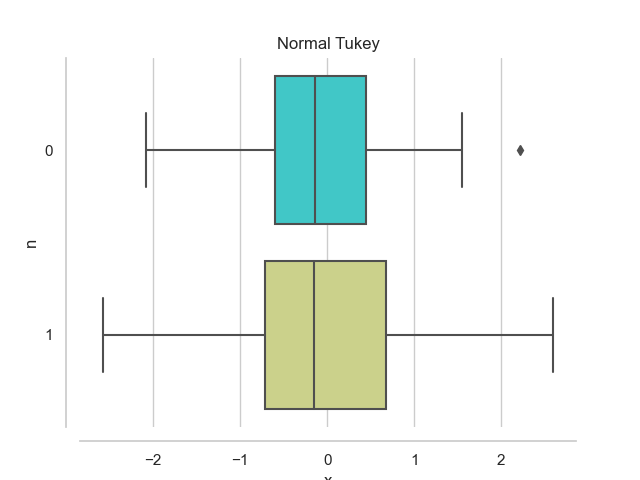
\includegraphics[scale=0.8]{NormalTukey.png}
\caption{Нормальное распределение}\label{figure1}
\end{center}
\end{figure}

\begin{figure}[!ht]
\begin{center}
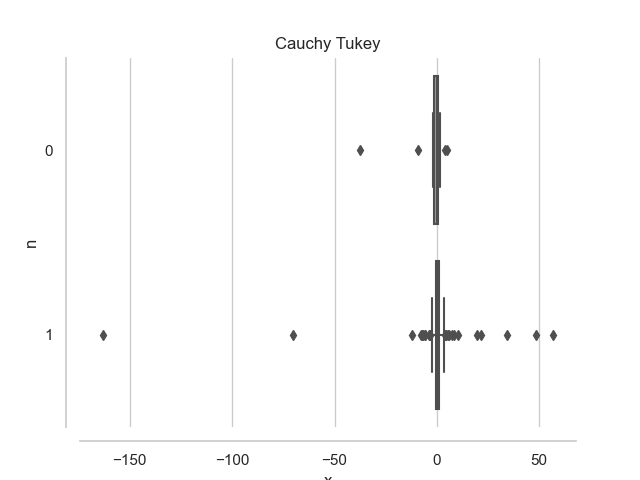
\includegraphics[scale=0.8]{CauchyTukey.png}
\caption{Распределение Коши}\label{figure2}
\end{center}
\end{figure}

\begin{figure}[!ht]
\begin{center}
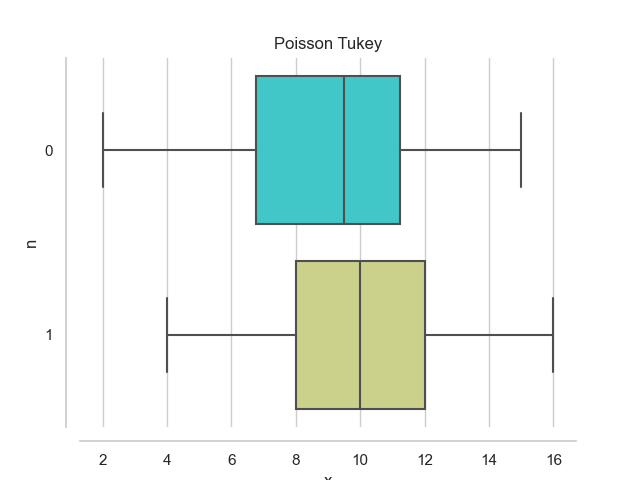
\includegraphics[scale=0.8]{PoissionTukey.png}
\caption{Распределение Пуассона}\label{figure4}
\end{center}
\end{figure}

\begin{figure}[!ht]
\begin{center}
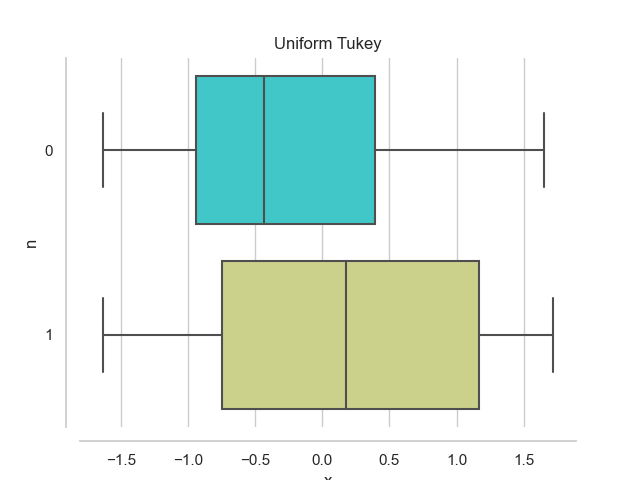
\includegraphics[scale=0.8]{UniformTukey.png}
\caption{Равномерное распределение}\label{figure5}
\end{center}
\end{figure}

~\\
~\\
~\\
~\\
~\\
~\\
~\\
~\\
~\\

\subsection{Доля выбросов}

\begin{table}[h!]
\begin{center}
\begin{tabular}{|c|c|}
\hline
Выборка & Доля выбросов \\
\hline
normal n = 20 & 0.05 \\
\hline
normal n = 100 & 0.01 \\
\hline
cauchy n = 20 & 0.15 \\
\hline
cauchy n = 100 & 0.13 \\
\hline
poisson n = 20 & 0.02 \\
\hline
poisson n = 100 & 0.01 \\
\hline
uniform n = 20 & 0 \\
\hline
uniform n = 100 & 0 \\
\hline


\end{tabular}
\caption{Доля выбросов}
\label{tabular:timesandtenses}
\end{center}
\end{table}

~\\
~\\
~\\
~\\
~\\
~\\
~\\
~\\
~\\

\subsection{Теоретическая вероятность выбросов}

\begin{table}[h!]
\begin{center}
\begin{tabular}{|c|c|c|c|c|c|}
\hline
Распределение & $Q^T_1$ & $Q^T_3$ & $X^T_1$ & $X^T_2$ & $P^T_B$ \\
\hline
Normal & -0.674 & 0.674 & -2.698 & 2.698 & 0.007\\
\hline
Cauchy & -1 & 1 & -4 & 4 & 0.156 \\
\hline
Poisson & 8 & 12 & 2 & 18 & 0.008\\
\hline
Uniform & -0.866 & 0.866 & -3.464 & 3.464 & 0 \\
\hline
\end{tabular}
\caption{Теоретическая вероятность выбросов}
\label{tabular:timesandtenses}
\end{center}
\end{table}



\subsection{Эмпирическая функция распределения}

\begin{figure}[!ht]
\begin{center}
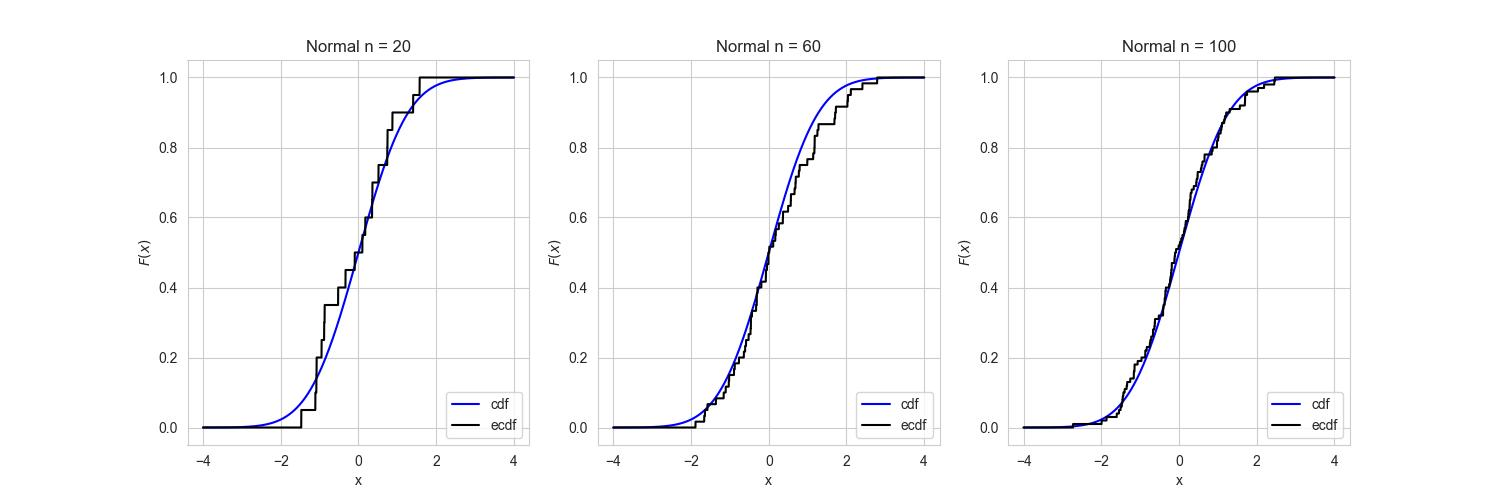
\includegraphics[scale=0.4]{NormalEmp.jpg}
\caption{Нормальное распределение}\label{figure1}
\end{center}
\end{figure}
~\\
~\\


\begin{figure}[!ht]
\begin{center}
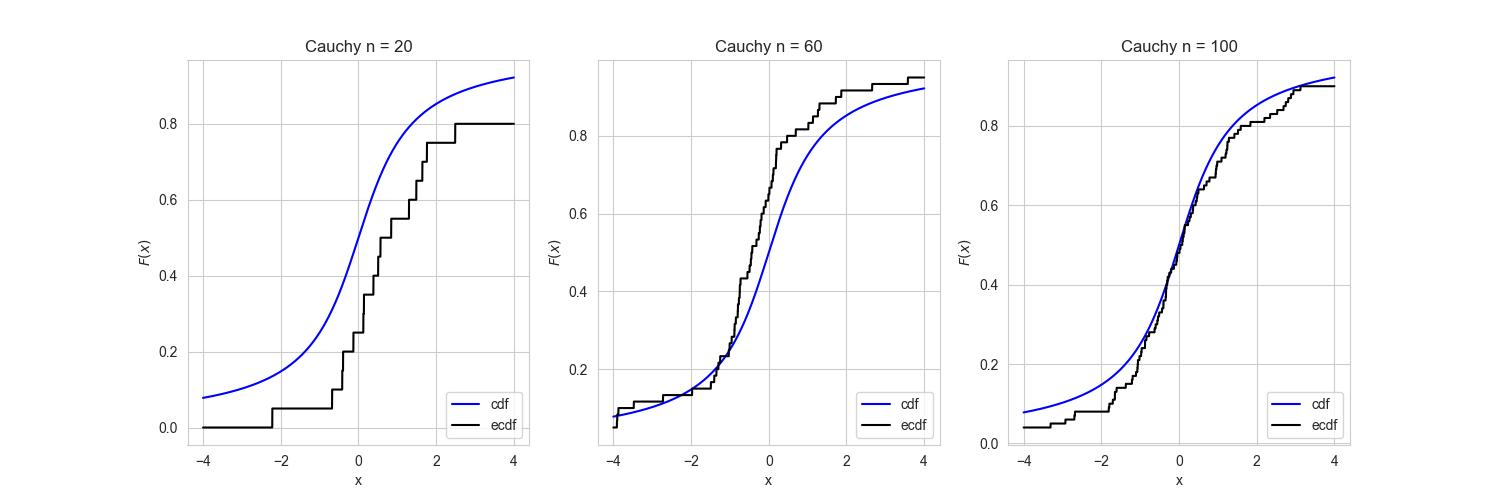
\includegraphics[scale=0.4]{CauchyEmp.jpg}
\caption{Распределение Коши}\label{figure2}
\end{center}
\end{figure}

\begin{figure}[!ht]
\begin{center}
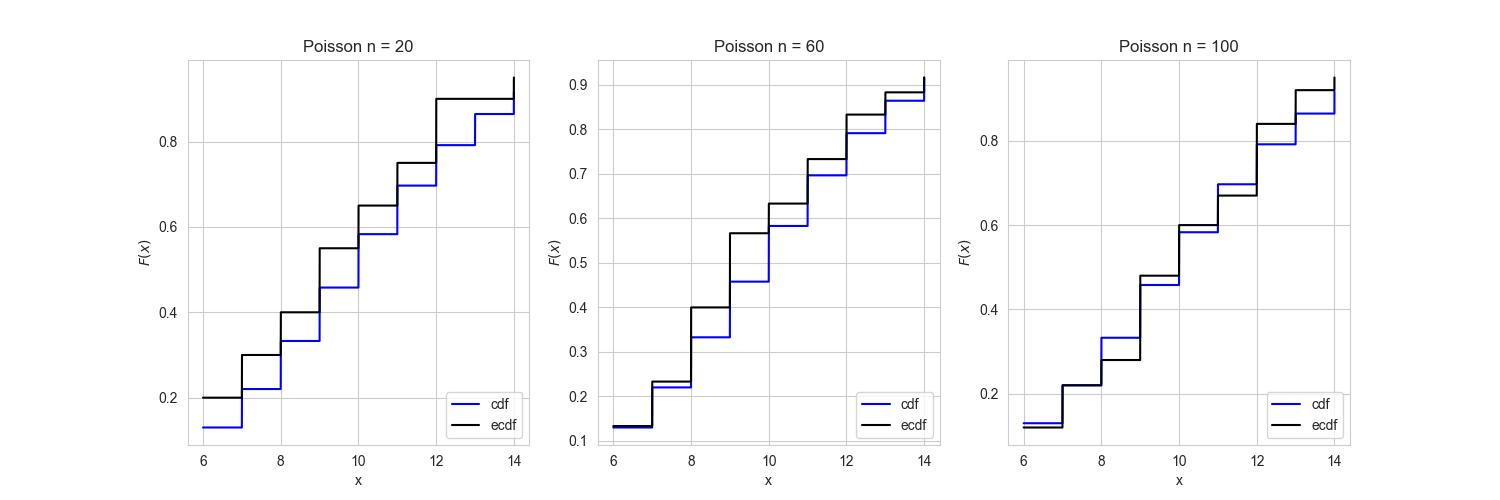
\includegraphics[scale=0.4]{PoissonEmp.jpg}
\caption{Распределение Пуассона}\label{figure4}
\end{center}
\end{figure}

\begin{figure}[!ht]
\begin{center}
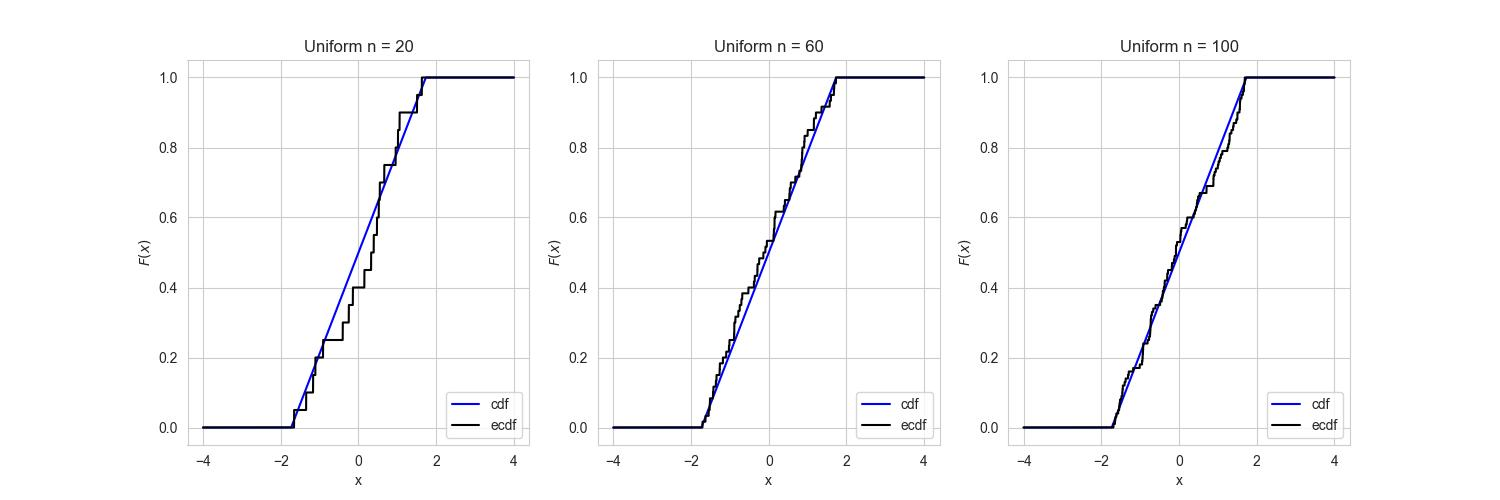
\includegraphics[scale=0.4]{UniformEmp.jpg}
\caption{Равномерное распределение}\label{figure5}
\end{center}
\end{figure}

~\\
~\\


\subsection{Ядерные оценки плотности распределения}
~\\


\begin{figure}[!ht]
\begin{center}
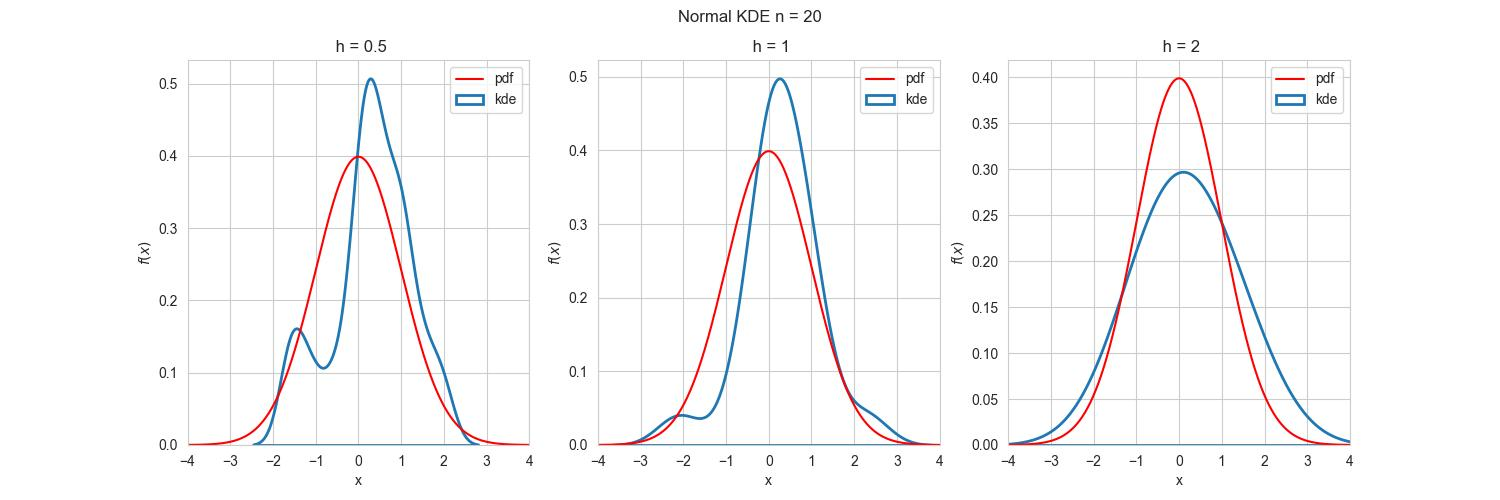
\includegraphics[scale=0.4]{Normal KDE20.jpg}
\caption{Нормальное распределение, n=20}\label{figure5}
\end{center}
\end{figure}

\begin{figure}[!ht]
\begin{center}
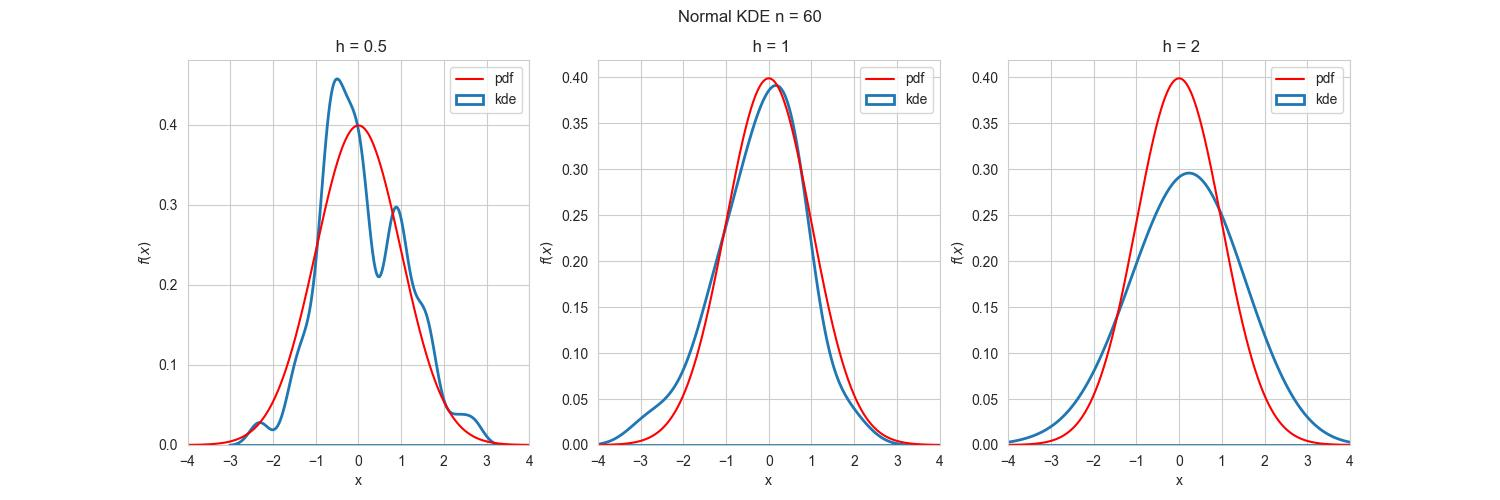
\includegraphics[scale=0.4]{Normal KDE60.jpg}
\caption{Нормальное распределение, n=60}\label{figure5}
\end{center}
\end{figure}

\begin{figure}[!ht]
\begin{center}
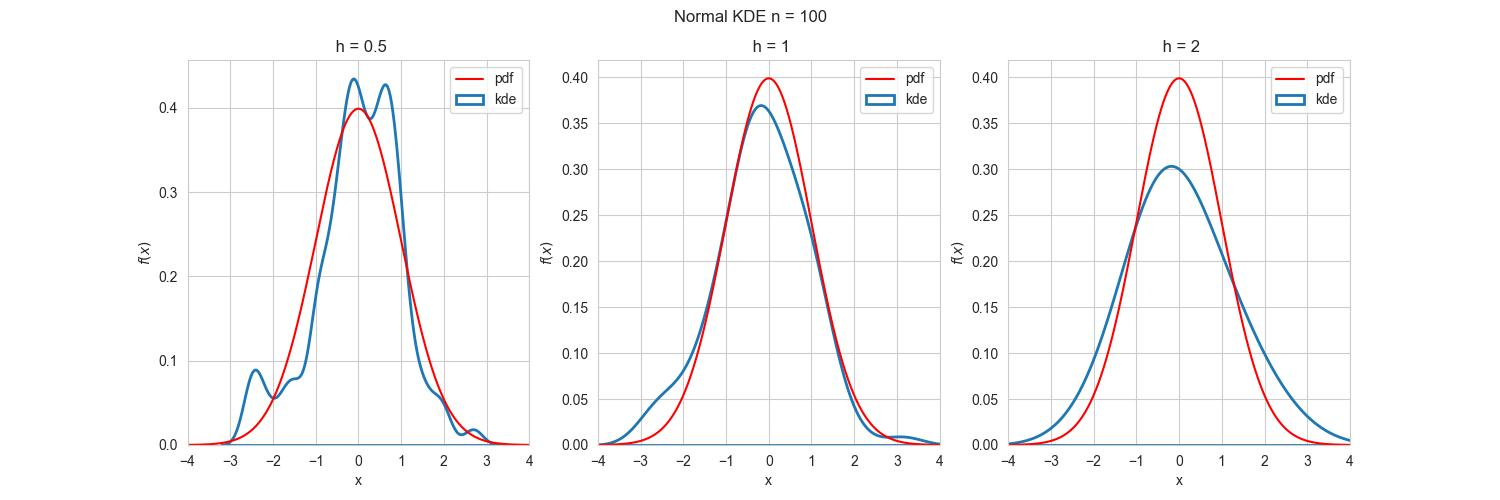
\includegraphics[scale=0.4]{Normal KDE100.jpg}
\caption{Нормальное распределение, n=100}\label{figure5}
\end{center}
\end{figure}
~\\


\begin{figure}[!ht]
\begin{center}
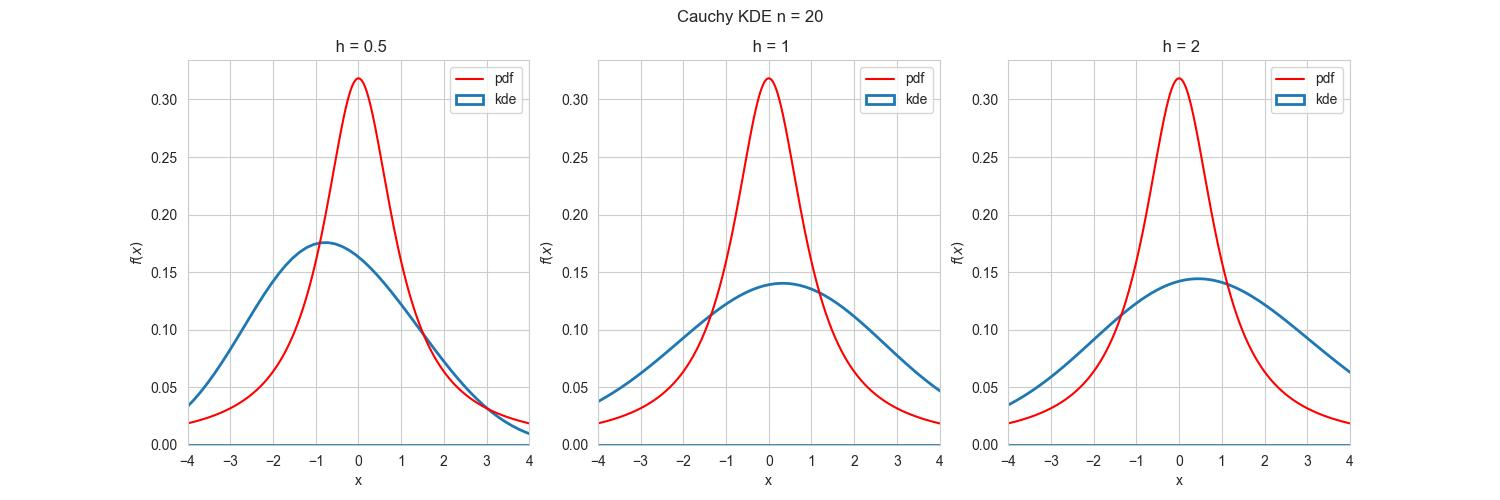
\includegraphics[scale=0.4]{Cauchy KDE20.jpg}
\caption{Распределение Коши, n=20}\label{figure2}
\end{center}
\end{figure}
~\\
~\\
~\\
~\\
~\\
~\\
~\\
~\\
~\\

\begin{figure}[!ht]
\begin{center}
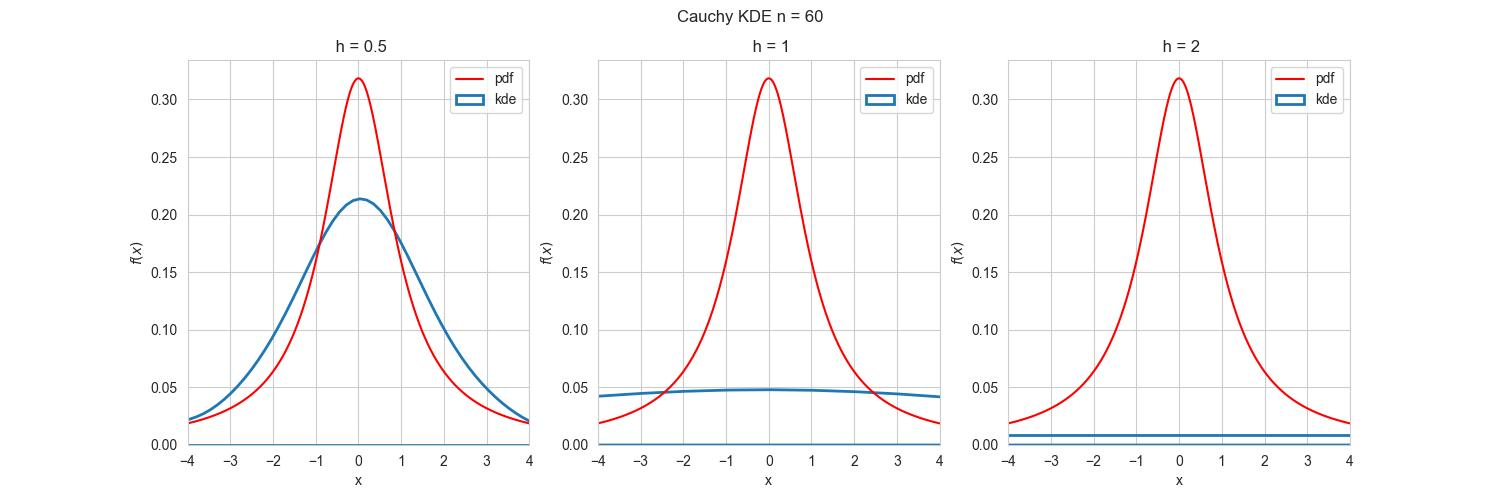
\includegraphics[scale=0.4]{Cauchy KDE60.jpg}
\caption{Распределение Коши, n=60}\label{figure2}
\end{center}
\end{figure}

\begin{figure}[!ht]
\begin{center}
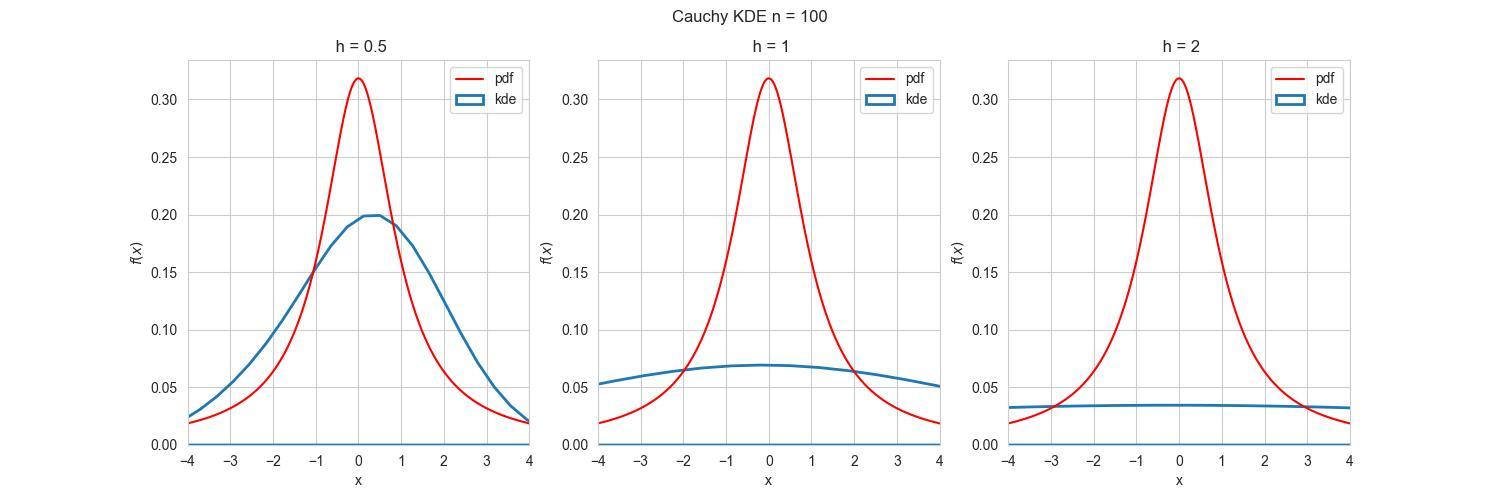
\includegraphics[scale=0.4]{Cauchy KDE100.jpg}
\caption{Распределение Коши, n=100}\label{figure2}
\end{center}
\end{figure}

\begin{figure}[!ht]
\begin{center}
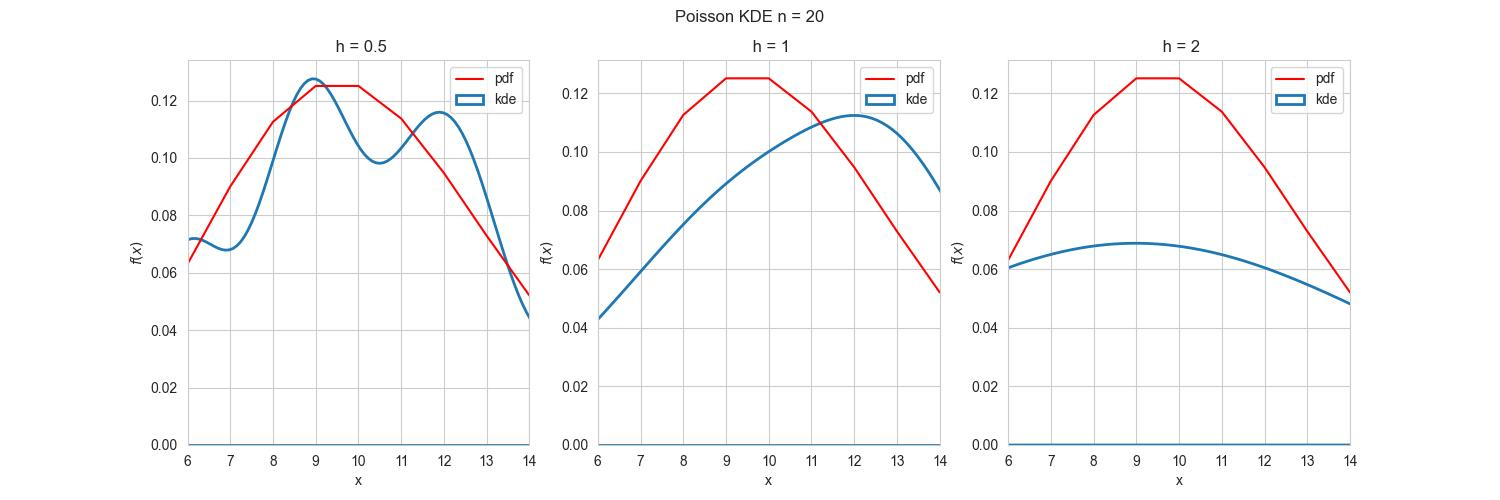
\includegraphics[scale=0.4]{Poisson KDE20.jpg}
\caption{Распределение Пуассона, n=20}\label{figure4}
\end{center}
\end{figure}

\begin{figure}[!ht]
\begin{center}
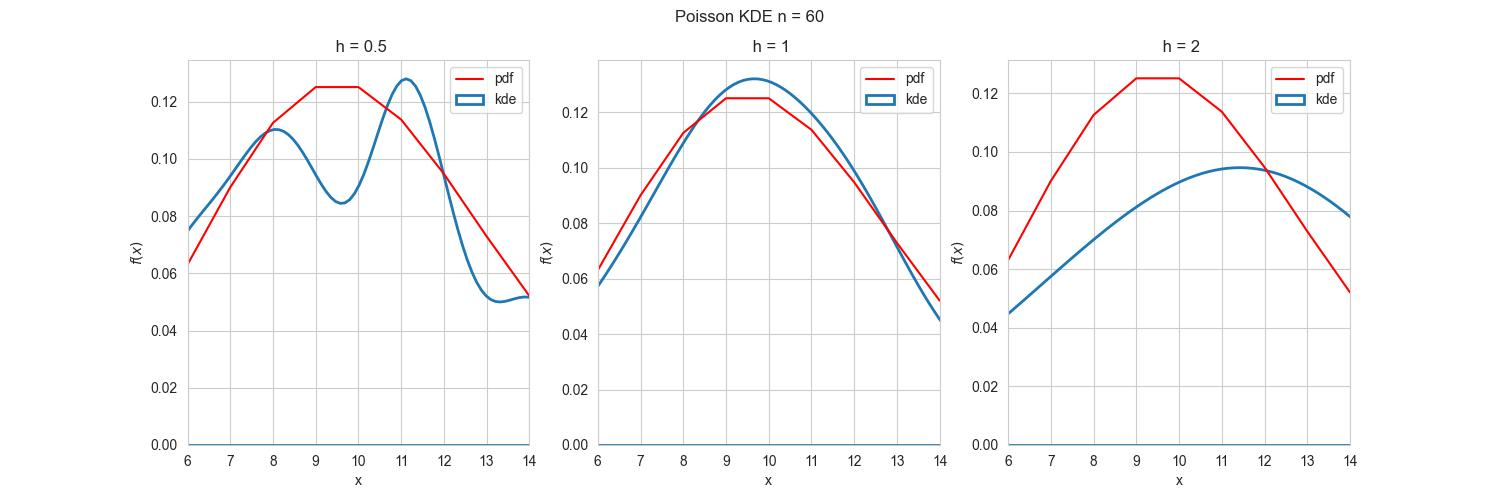
\includegraphics[scale=0.4]{Poisson KDE60.jpg}
\caption{Распределение Пуассона, n=60}\label{figure4}
\end{center}
\end{figure}

\begin{figure}[!ht]
\begin{center}
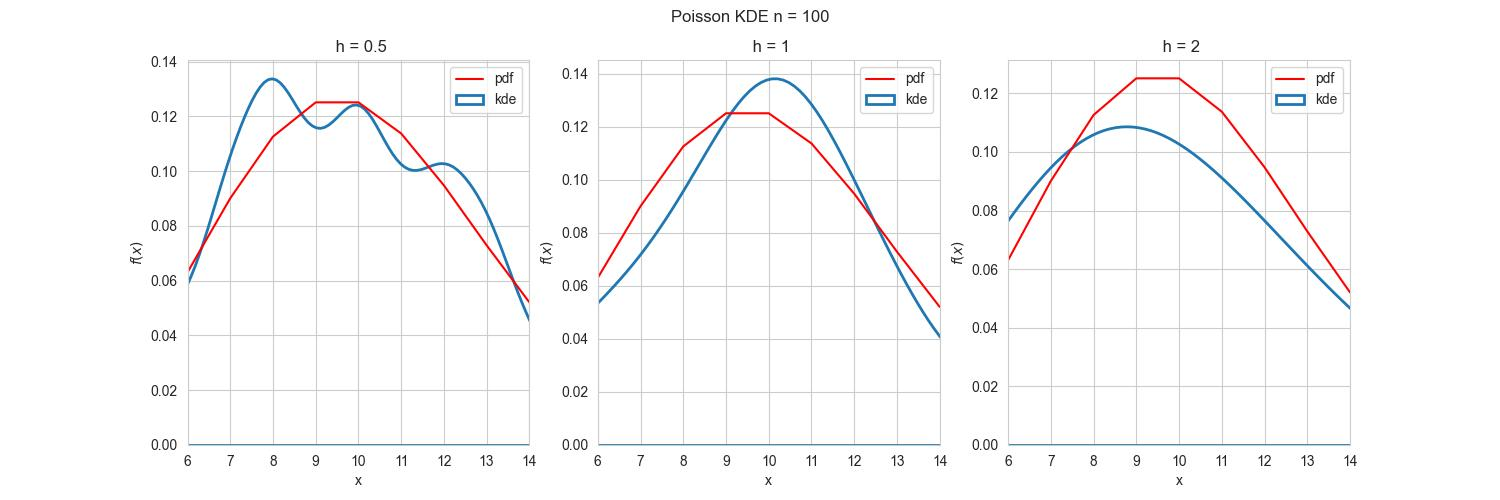
\includegraphics[scale=0.4]{Poisson KDE100.jpg}
\caption{Распределение Пуассона, n=100}\label{figure4}
\end{center}
\end{figure}

\begin{figure}[!ht]
\begin{center}
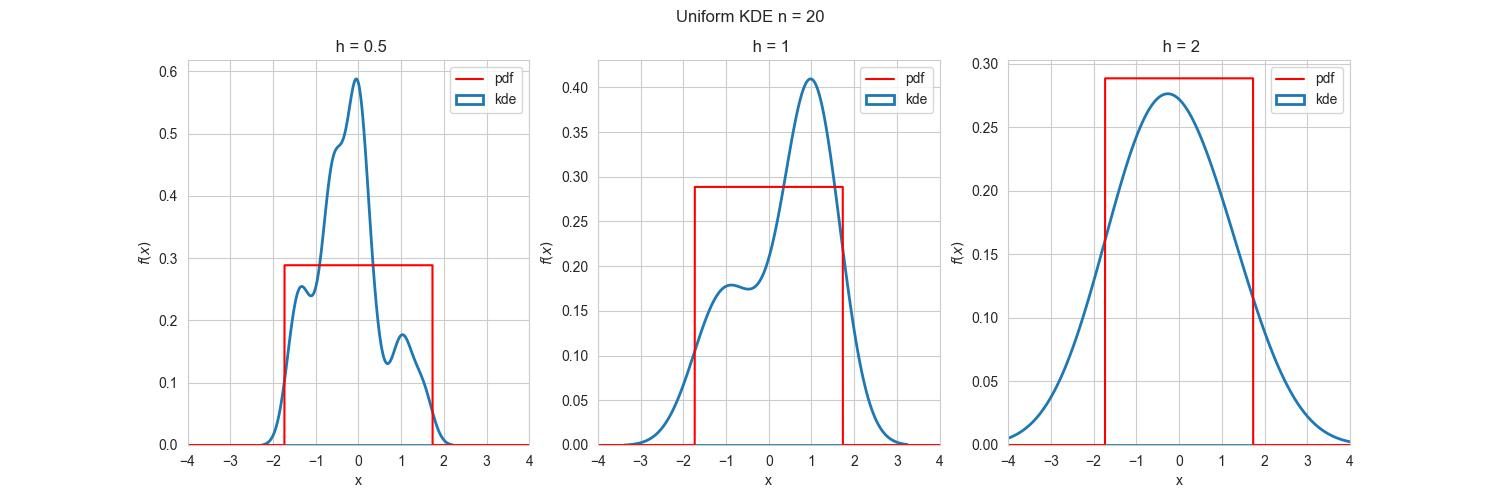
\includegraphics[scale=0.4]{Uniform KDE20.jpg}
\caption{Равномерное распределение, n=20}\label{figure5}
\end{center}
\end{figure}

\begin{figure}[!ht]
\begin{center}
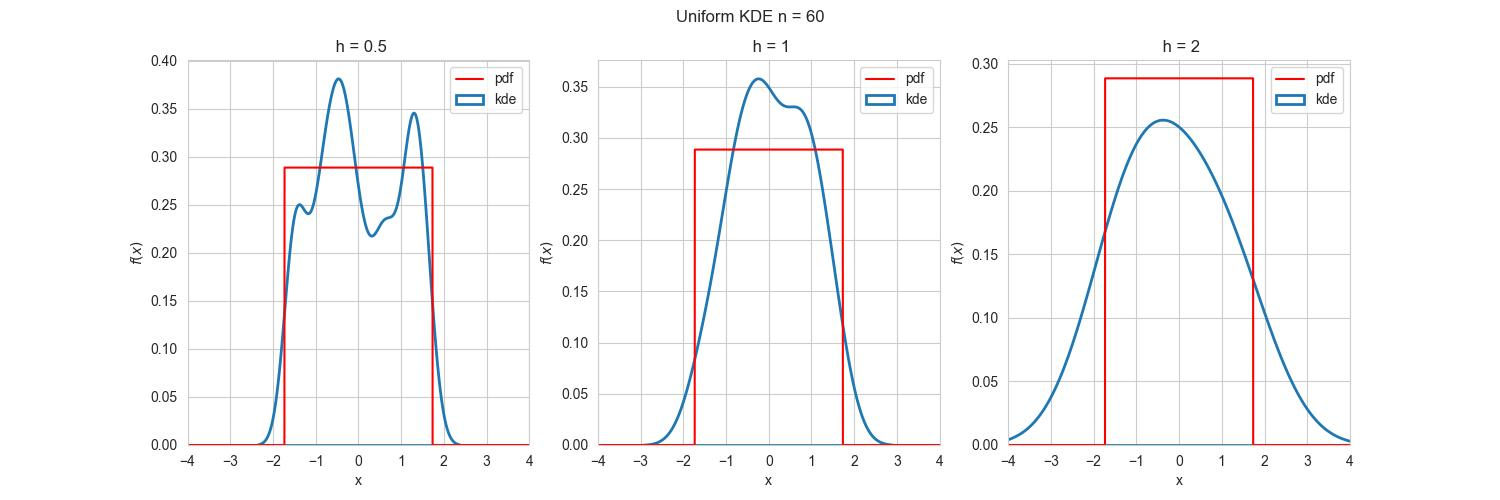
\includegraphics[scale=0.4]{Uniform KDE60.jpg}
\caption{Равномерное распределение, n=60}\label{figure5}
\end{center}
\end{figure}

~\\
~\\
~\\
~\\
~\\
~\\
~\\
~\\
~\\

\begin{figure}[!ht]
\begin{center}
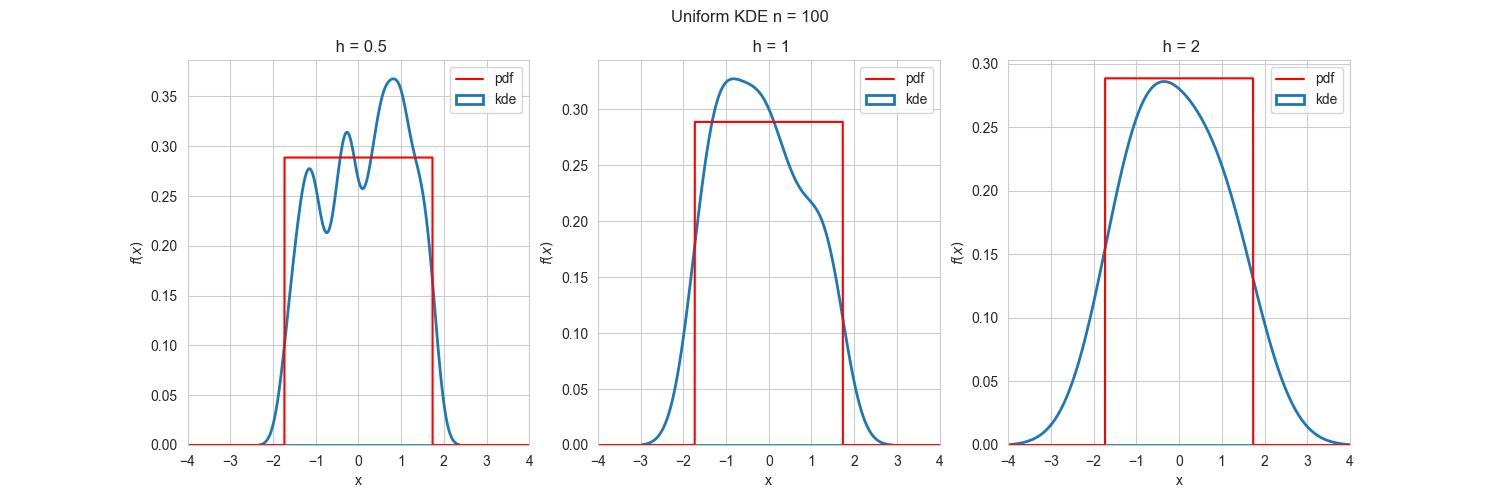
\includegraphics[scale=0.4]{Uniform KDE100.jpg}
\caption{Равномерное распределение, n=100}\label{figure5}
\end{center}
\end{figure}

~\\
~\\
~\\
~\\
~\\
~\\
~\\
~\\
~\\
~\\
~\\
~\\
~\\
\newpage

\section{Обсуждение}

\subsection{Гистограммы}
По результатам проделанной работы можем сделать вывод о том, что чем
больше выборка для каждого из распределений, тем ближе ее гистограмма
к графику плотности вероятности того закона, по которому распределены
величины сгенерированной выборки. Чем меньше выборка, тем менее она
показательна - тем хуже по ней определяется характер распределения величины.
Также можно заметить, что максимумы гистограмм и плотностей распределения почти нигде не совпали. Также наблюдаются всплески гистограмм,
что наиболее хорошо прослеживается на распределении Коши.

\subsection{Характеристики положения и рассеяния}
Исходя из данных, приведенных в таблицах, можно судить о том, что дисперсия характеристик рассеяния для распределения Коши является некой
аномалией: значения слишком большие даже при увеличении размера выборки - понятно, что это результат выбросов, которые мы могли наблюдать
в результатах предыдущего задания.

\subsection{Доля и теоретическая вероятность выбросов}
По данным, приведенным в таблице, можно сказать, что чем больше выборка, тем ближе доля выбросов будет к теоретической оценке. Снова доля
выбросов для распределения Коши значительно выше, чем для остальных
распределений. Равномерное распределение же в точности повторяет теоретическую оценку - выбросов мы не получали.
Боксплоты Тьюки действительно позволяют более наглядно и с меньшими
усилиями оценивать важные характеристики распределений. Так, исходя
из полученных рисунков, наглядно видно то, что мы довольно трудоёмко
анализировали в предыдущих частях.

\subsection{Эмпирическая функция и ядерные оценки плотности распределения}
Можем наблюдать на иллюстрациях с э. ф. р., что ступенчатая эмпирическая функция распределения тем лучше приближает функцию распределения реальной выборки, чем мощнее эта выборка. Заметим так же, что для
распределения Пуассона и равномерного распределения отклонение функций друг от друга наибольшее.
Рисунки, посвященные ядерным оценкам, иллюстрируют сближение ядерной оценки и функции плотности вероятности для всех $h$ с ростом размера
выборки. Для распределения Пуассона наиболее ярко видно, как сглаживает отклонения увеличение параметра сглаживания $h$.
В зависимости от особенностей распределений для их описания лучше подходят разные параметры $h$ в ядерной оценке: для равномерного распределения и распределения Пуассона лучше подойдет параметр $h=2h_n$, для
распределения Лапласа $-h=\frac{h_n}{2}$, а для нормального и Коши $-h=h_n$.
Такие значения дают вид ядерной оценки наиболее близкий к плотности,
характерной данным распределениям.
Также можно увидеть, что чем больше коэффициент при параметре сглаживания $\widehat{h}_n$, тем меньше изменений знака производной у аппроксимирующей функции, вплоть до того, что при $h=2h_n$ функция становится унимодальной на рассматриваемом промежутке. Также видно, что при $h=2h_n$
по полученным приближениям становится сложно сказать плотность вероятности какого распределения они должны повторять, так как они очень
похожи между собой.

\newpage

\section{Приложение}
Код программы GitHub: https://github.com/KsenErem/MatStat
\end{document}
